\documentclass{sig-alternate}
\usepackage{tikz}
  \def\firstcircle{(90:1.75cm) circle (2.5cm)}
  \def\secondcircle{(210:1.75cm) circle (2.5cm)}
  \def\thirdcircle{(330:1.75cm) circle (2.5cm)} 
\usepackage{comment}
\usepackage{cite}
\usepackage[shortlabels]{enumitem} 
\usepackage{amsmath}
\usepackage{url}
\usepackage{balance}
\newcommand{\bi}{\begin{itemize}[leftmargin=0.4cm]}
\newcommand{\ei}{\end{itemize}}
\newcommand{\be}{\begin{enumerate}}
\newcommand{\ee}{\end{enumerate}}
\newcommand{\tion}[1]{\S\ref{sect:#1}}
\newcommand{\fig}[1]{Figure~\ref{fig:#1}}
\newcommand{\eq}[1]{Equation~\ref{eq:#1}}
\setlist{nolistsep,leftmargin=5mm}
%\usepackage[pdftex]{graphicx}
\usepackage{program}
\newcommand{\Sample}{{\bf SAMPLE}}
\newcommand{\PEEKING}{{\bf PEEKING2}}
%\usepackage[table]{xcolor}
\definecolor{darkgreen}{rgb}{0,0.3,0}
\definecolor{Gray}{rgb}{0.88,1,1}
\definecolor{Gray}{gray}{0.85}
\definecolor{Blue}{RGB}{0,29,193}
\usepackage{colortbl}
\usepackage{picture}
\usepackage{url}
\usepackage{hyperref}
\usepackage{listings}
\DeclareMathOperator*{\argmin}{arg\,min} 
\DeclareMathOperator*{\argmax}{arg\,max}
\definecolor{lightgray}{gray}{0.8}
\definecolor{darkgray}{gray}{0.6}
\definecolor{Gray}{gray}{0.95}
\definecolor{LightGray}{gray}{0.975}

\definecolor{Code}{rgb}{0,0,0}
\definecolor{Decorators}{rgb}{0.5,0.5,0.5}
\definecolor{Numbers}{rgb}{0.5,0,0}
\definecolor{MatchingBrackets}{rgb}{0.25,0.5,0.5}
\definecolor{Keywords}{rgb}{0,0,1}
\definecolor{self}{rgb}{0,0,0}
\definecolor{Strings}{rgb}{0,0.63,0}
\definecolor{Comments}{rgb}{0,0.63,1}
\definecolor{Comments}{rgb}{0.5,0.5,0.5}
\definecolor{Backquotes}{rgb}{0,0,0}
\definecolor{Classname}{rgb}{0,0,0}
\definecolor{FunctionName}{rgb}{0,0,0}
\definecolor{Operators}{rgb}{0,0,0}
\definecolor{Background}{rgb}{1,1,1}
\lstnewenvironment{code}[1]{
\lstset{
mathescape,
numbers=left,
numberstyle=\scriptsize,
stepnumber=1,
numbersep=0.5em,
xleftmargin=1em,
framextopmargin=2em,
framexbottommargin=2em,
showspaces=false,
showtabs=false,
showstringspaces=false,
tabsize=2,
% Basic
basicstyle=\ttfamily\scriptsize,
backgroundcolor=\color{Background},
language=Python,
% Comments
commentstyle=\color{Comments}\slshape,
% Strings
stringstyle=\color{Strings},
morecomment=[s][\color{Strings}]{"""}{"""},
morecomment=[s][\color{Strings}]{'''}{'''},
% keywords
morekeywords={[1]import,from,class,def,for,while,if,is,in,elif,else,not,and,or,print,break,continue,return,True,False,None,access,as,,del,except,exec,finally,global,import,lambda,pass,print,raise,try,assert, dot, norm, zip, sorted},
keywordstyle={[1]\color{Code}\bfseries},
% additional keywords
morekeywords={[3]fastmap,Slope,bPruning,clister,train,leafs,weightedFeatures,HOW,envy, score,kNN,contrastSet,exemplar,Prune, FSel, exemplar,nearestSlope,dist,displace,geometry,splitAcross2Points,leaves,How,nearest,bPruning,Stats,divide,recurse,weight1,project, furthest, split,WHERE,clusterer, getContours,envied, fWeight, nearestContour, projection, mutate, HERE, knn},
keywordstyle={[3]\color{Keywords}\bfseries},
morekeywords={[2]@invari},
keywordstyle={[2]\color{Decorators}\slshape},
emph={self},
emphstyle={\color{self}\slshape},
firstnumber=last
%
}}{}
 
\newcommand{\G}{\cellcolor{green}}
\newcommand{\Y}{\cellcolor{yellow}}

\newcommand{\quart}[4]{\begin{picture}(100,4)%1
{\color{black}\put(#3,2){\circle*{4}}\put(#1,2){\line(1,0){#2}}}\end{picture}}


\definecolor{MyDarkBlue}{rgb}{0,0.08,0.45} 
\newenvironment{changed}{\par\color{MyDarkBlue}}{\par}
%\newenvironment{changed}{\par}{\par}

\newcommand{\ADD}[1]{\textcolor{MyDarkBlue}{{\bf #1}}}
\usepackage{times}
\pagenumbering{arabic} 
\begin{document}  
\conferenceinfo{ISCE}{'16 Austin, Texas}

\title{Learning Useful Changes\\(to Reduce Runtimes and Software Defects)}
\numberofauthors{3} 
\author{
\alignauthor 
Rahul~Krishna,~Tim Menzies,~Xipeng~Shen \\
       \affaddr{Com. Sci., NC State, USA}\\
       {\{i.m.ralk,~tim.menzies,\\xipengshen\}@gmail.com}
\alignauthor
Naveen   Lekkalapudi\\
 \affaddr{Software Consultant } \\ 
       \affaddr{Washington D.C.}\\ 
       {navek91@gmail.com}
\alignauthor
Lucas Layman \\
       \affaddr{Fraunhofer CESE  } \\ 
       \affaddr{College Park, USA}\\ 
       {llayman@fc-md.umd.edu}
\setlength{\columnsep}{7mm}
}
\maketitle
\begin{abstract}
 As business users demand more insightful
 analytics, data scientists need to change
 their tools. Instead of merely predicting 
 some result, they also need tools that generate ``plans'';
 i.e. specific suggestions on  how to change values in order to
 improve on some predicted value.
 
This paper is aims to study such planners. The planners fall into three broad categories (1) Cluster specific planners (K Nearest Neighbors); (2) Instance specific planners (HOW); (3) Decision Tree based planners. These planners are employed as tools for proposing changes to independent
 variables in order to improve on 
 the predictions of the dependent variables. Unlike other approaches
 for learning optimizations to software, these planners do not require
 an underlying model of the domain. Also, these plans
 are designed to result in {\em minimal displacement}
 to current practice.
 
 This paper uses these learners to learn methods
 to reduce defects and decrease program runtime.
 For the test data of this paper, those improvements   reduce
 the expected values of defect counts and  runtimes to    
 45\%,61.5\%  (median) and 22\%,6\% (best case) of the initial values, respectively.
\end{abstract}
\section{Introduction}
We propose a novel {\em planning} approach called CROSSTREES for learning changes to a software system
such that its performance ``improves'', according to some measure. For  case 
studies, we apply CROSSTREES to   (1)~reduce the predicted number
of defects and (2)~reduce the runtimes of five system. 

The approach discussed here is novel since most data miners used in software analytics
comment on ``what is'' and not ``what to do''. For example, a clustering
algorithm might find clumps of similar examples, but does not comment on the minimal
change(s) required to move from clump to clump.

Our approach is important for two reasons. Firstly, business users now demanding analytics tools that support a business-level interpretation of their data. At a panel on software analytics at ICSE`12, industrial practitioners lamented the state of the art in data mining and software engineering~\cite{menzies12a}. Panelists commented that ``prediction is all well and good, but what about decision making?''. That is, these panelists are more interested in the interpretations and follow-up that occurs after the mining, rather than just the mining itself. For example:
\bi
\item
Instead of just accepting {\em predictions} on how many software defects to expect, business users might now demand a {\em plan} to reduce the likelihood of those defects.
\item
Instead of just accepting {\em predictions} on the runtime time of their software, business users might now demand a {\em plan} to reduce that runtime. 
\ei
A second reason for the importance of our approach is, as shown below,
when asked how to change a project in order to achieve a result, it is surprisingly
difficult to use standard methods (e.g. clustering) to find those changes.
In the case study that motivated this paper, we how  standard data mining methods
can generate  seemingly
useful insights, but which are in fact completely ineffectual. On the other hand,
using CROSSTREES, we can propose changes that significantly reduce:
\bi
\item The  defects found  in Jureczko et al.'s    JAVA systems~\cite{jureczko10}.
\item The runtime of the  software    configured by  Seigmund et al.~\cite{sven12}.
\ei 
Since CROSSTREES is a somewhat novel algorithm, we present it in tutorial form.
The next section walks the reader through a sequence of approaches that start
with a standard clustering algorithm, and progresses on to CROSSTREES. The second
half of the paper then presents an extensive evaluation of CROSSTREES on 
the Jureczko  and Seigmund data sets. This is followed by notes on related work
and validity.

\section{ Methods for Learning Changes}
 This paper experimentally compares four methods for inputting software project data and outputting
 recommendations on what to change.
 For case studies that illustrate how this method works, we use data from Jureczko et al.'s object-oriented JAVA systems~\cite{jureczko10} (shown in \fig{ck} and \fig{jd}) and
  software system   configuration data from by  Seigmund et al.~\cite{sven12} (see \fig{cpm}).
  
  The Jurecko data records number of known defects for each class, where the classes are described in terms of
  nearly two dozen metrics such as number of children, lines of code, etc.
  
  The Seigmund data records the runtime of compiled systems. To generate that data, Seigmund et al. perturbed
  the configuration parameters in the Makefiles of six systems: Apache, SQLite, LLVM, x264 and two versions of the
  Berkeley database (one written in ``C'' and one in Java). To ensure that the perturbations
  were valid, the option space was modeled as a tree that included knowledge of what
  options were mandatory, optional, or were alternatives (see \fig{bdbc}).
  Given those perturbations, the systems were then compiled and 
  Seigmund et al. recorded how long each perturbation took to complete a test suite. 
  

\begin{figure*}[t!]
	\renewcommand{\baselinestretch}{0.8}\begin{center}
		{\scriptsize
			\begin{tabular}{c|l|p{4.7in}}
				amc & average method complexity & e.g. number of JAVA byte codes\\\hline
				avg\, cc & average McCabe & average McCabe's cyclomatic complexity seen
				in class\\\hline
				ca & afferent couplings & how many other classes use the specific
				class. \\\hline
				class. \\\hline
				cam & cohesion amongst classes & summation of number of different
				types of method parameters in every method divided by a multiplication
				of number of different method parameter types in whole class and
				number of methods. \\\hline
				cbm &coupling between methods &  total number of new/redefined methods
				to which all the inherited methods are coupled\\\hline
				cbo & coupling between objects & increased when the methods of one
				class access services of another.\\\hline
				ce & efferent couplings & how many other classes is used by the
				specific class. \\\hline
				dam & data access & ratio of the number of private (protected)
				attributes to the total number of attributes\\\hline
				dit & depth of inheritance tree &\\\hline
				ic & inheritance coupling &  number of parent classes to which a given
				class is coupled (includes counts of methods and variables inherited)
				\\\hline
				lcom & lack of cohesion in methods &number of pairs of methods that do
				not share a reference to an case variable.\\\hline
				locm3 & another lack of cohesion measure & if $m,a$ are  the number of
				$methods,attributes$
				in a class number and $\mu(a)$  is the number of methods accessing an
				attribute, 
				then
				$lcom3=((\frac{1}{a} \sum, j^a \mu(a, j)) - m)/ (1-m)$.
				\\\hline
				loc & lines of code &\\\hline
				max\, cc & maximum McCabe & maximum McCabe's cyclomatic complexity seen
				in class\\\hline
				mfa & functional abstraction & number of methods inherited by a class
				plus number of methods accessible by member methods of the
				class\\\hline
				moa &  aggregation &  count of the number of data declarations (class
				fields) whose types are user defined classes\\\hline
				noc &  number of children &\\\hline
				npm & number of public methods & \\\hline
				rfc & response for a class &number of  methods invoked in response to
				a message to the object.\\\hline
				wmc & weighted methods per class &\\\hline
				\rowcolor{lightgray}
				nDefects & raw defect counts & Numeric: number of defects found in post-release bug-tracking systems.\\
				\rowcolor{lightgray}
				defect & defects present? & Boolean: if {\em nDefects} $>0$ then {\em true} else {\em false}
			\end{tabular}
		}
	\end{center}
	\caption{OO measures used in our defect data sets.  Last lines, shown in \textcolor{gray} denote the dependent variables.}\label{fig:ck}
\end{figure*}

 \begin{figure}
 \scriptsize
 \begin{center}
 \begin{tabular}{r|rr}
 data set & cases & \% defective\\\hline
  ant &947& 22\\
  camel& 1819& 19\\
 jedit& 1257& 2\\
 ivy &352& 11\\
 log4j& 244 &92\\
 lucebe &442 &59\\
 poi& 936 &64\\
 synapse &379 &34\\
 velocity& 410& 34\\
 xalan& 2411& 99\\
 xerces &1055& 74
 \end{tabular}
 \end{center}
 \caption{The Jureczko data sets (columns in the format of \fig{ck}).}\label{fig:jd}
 \end{figure}
 
 \begin{figure}[!t]
\scriptsize
\begin{tabular}{llllll}
  \hline
  \rowcolor{lightgray}
Project & Domain & Lang. & LOC & Features & Config\\\hline
Berkeley DB CE & Database & C & 219,811 & 18 & 2560\\
Berkeley DB JE & Database & Java & 42,596 & 32  & 400\\
Apache & Web Server & C & 230,277 & 9 & 192\\
SQLite & Database & C & 312,625 & 39 & 3,932,160\\
LLVM & Compiler & C++ & 47,549 & 11 & 1024\\
x264 & Video Enc. & C& 45,743 & 16 & 1152\\\hline
\end{tabular}
 
\caption{Seigmund data sets: details on the data sets.
For SQLite, the data  contains 4,553 configurations for prediction modeling and 100 additional random configurations for prediction evaluation, see \cite{vapp}.}\label{fig:cpm}
\end{figure}

\begin{figure}[!t]
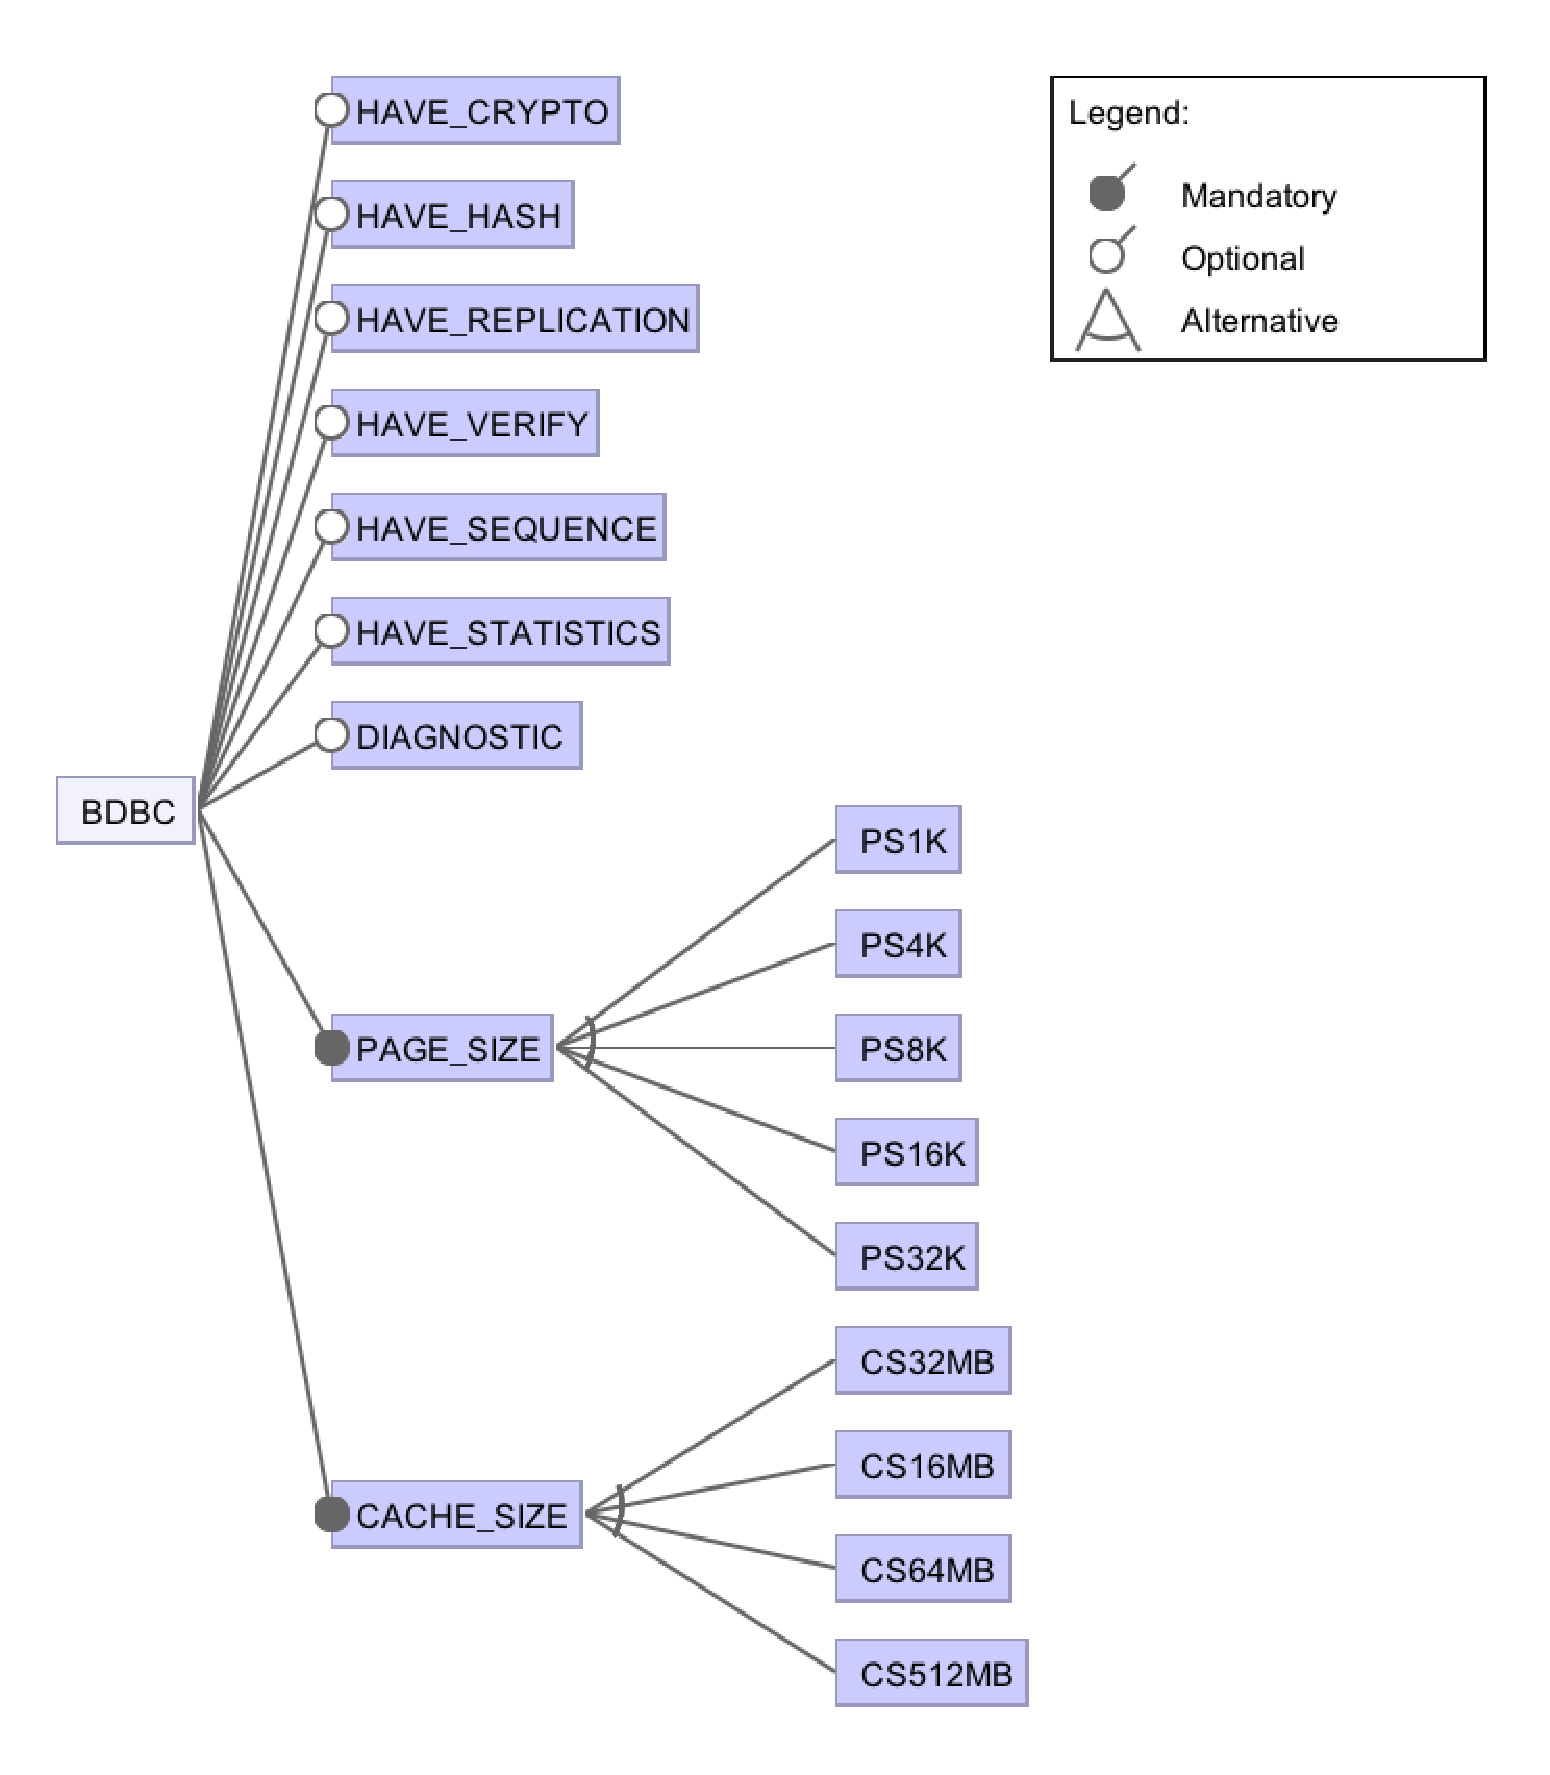
\includegraphics[width=1\linewidth]{_figs/BDBC.eps}
\caption{Feature model for the Berkeley database (``C'' version). }\label{fig:bdbc}
\end{figure}

Research has shown that given the above data, it is possible to build
predictors for defective classes (in the Jureczko data) or for the runtime
of a compiled system (in the Seigmund data) (e.g. see ~\cite{sven12,nam13,he13,peters13,Menzies2013:local,me09b,me11f,me07b}).
This paper is about the next step {\em after} prediction. We envisonage as scenario
where business users are presented a prediction and they do not like what they see; e.g. the runtimes are too long of the number of defects is too high. Such users will
then ask a {\em planning}  question; i.e. ``what can we change to do better than that?'' The rest of this paper
defines and explores four methods for generating those plans.

\subsection{Method1: Centroid Deltas}


In the summer of 2011 and 2012, one of us (Menzies) spent two months
	working on-site at Microsoft Redmond,
	observing data mining analysts.  In that study, he took special
	note about how Microsoft's data scientists
	discussed the results of their data mining sessions with  business users. 
	
	One surprising observation was how  
	little time was spent by business users 
	inspecting  of the output of standard data miners. Prior to that visit,
	we had the mistaken impression that   decision trees,
	clustering algorithms, etc were useful ``off-the-shelf''; i.e    business
	users would inspect and understand the output of those tools.
	
Standard data mining tools are not necessarily the best tool for supporting that dialogue.
Menzies found that he had to do considerable work pre-processing data mining output
prior to the weekly briefing meetings for the business users. Initially,
that pre-processing was just clustering. This evolved into feature selection and finally
the a case-based reasoning tool called HOW.  


	
	as compared to another process, which we call {\em peeking}.
	In {\em peeking}, analysts and users spend much time
	inspecting and discussing small samples of either raw or exemplary or synthesized project data.  Further, very little of those discussions were  focused on classification
	(the addition of a labels to some unlabelled data). Rather, much time
	was spent in those meetings discussing {\em what to do next}; i.e. trying
	to determine what could be altered to better improve some business outcome.
	
	That   Microsoft  study found two common ``peeking'' methods.
	In {\em data engagement meetings},
	users debated the implications of data
	displayed on a screen. In this way, users
	engaged with the data and with each other by
	monitoring each others' queries and check each others'
	conclusions.
	
	Another data analysis pattern observed
	at Microsoft was  {\em cluster + contrast} in which
	data is  reduced to a few
	clusters. Users are then just shown the delta between those
	clusters. While contrasting, if feature values are
	the same in both clusters, then these were pruned from
	the reports to the user. In this way, very large
	data sets can be shown on one PowerPoint
	slide. Note that {\em cluster+contrast} is a tool that can be usefully employed within
	{\em data engagement meetings}.
	
	
	Cluster+contrast and engagement
	meetings are common practices at Microsoft. Yet  these methods had never been rigorously studied or certified.
	For both those reasons,
	we reflected over those tools to discover and analyze their
	underlying process. The result was HOW~\cite{howase}: a tool
	that combines (a)~feature selection; (b)~centroid generation from   clusters;
	(c)~contrast methods between centroids.
	While method (a) is widely used (e.g.~\cite{Menzies2010}),
	to the best of our knowledge, this combination of (abc) has not been thoroughly explored before.

This paper assesses two methods  for ``peeking'': a model-based method called DTREE and an instance-based method   called HOW. 
DTREE were first developed by Lekkalapudi and Menzies to  explaining results from multi-objective optimizers~\cite{nva14}. This paper is the first
to apply DTREE to defect prediction and contrast set learning. Also, that prior work evaluated
DTREE against multi-objective optimizers and not   instance-based methods.

This paper uses three criteria to assess the value of HOW and DTREE for
learning actionable analytics:
\be
\item
A planning system needs to be {\em effective}; i.e. if its recommendations
are applied then some statistically significant change should be observed.
To predict the number of defects in a data set before and after applying our changes,
we build a    prediction system (built by data mining; specifically: Random Forest). Note that this
predictor was built from some hold-out data (i.e. from  different data than that used
to build the predictor).
\item
Any  conclusion made to a business user must be understandable;
it must generate {\em succinct} changes.  
\item
Recommendations should be {\em stable}; i.e. they shouldn't widely vary due to minor changes in the data. Hence, in our experiments, we will add a little randomness to our analysis then report results across 20 repeated runs. 
\ee
We will find that
 {\em effectiveness} of DTREE and HOW are similar, but   DTREE wins on {\em succinctness} and {\em stability}.

\section{Cluster and Contrast}
\label{clust_contrast}
A recurring data analysis pattern in this paper is $cluster+contrast$. The data is distilled into a few clusters using a clustering scheme. Then lessons are inferred by studying the differences between these clusters. These lessons are used to generate rules that can be applied in any context.

\subsection{Clustering}
There are a wide variety of clustering methods to choose from. A study by Ganesan~\cite{div14} explored different clustering methods for software engineering data using the effort and defect data from the PROMISE repository~\cite{promise}. In that study methods such as WHERE, K-Means, mini-batch-K-Means, DBScan, EM, and Ward were investigated. The results of the study showed that the size and number of clusters is more important that the specifics of the techniques used. 

For this purposes of this work, we have chosen WHERE, a clustering scheme which is capable of generating at least $\sqrt{N}$ clusters given $N$ instances. In addition to this, WHERE has been shown to run fast while ignoring spurious dimensions~\cite{menzies2013}. This is particularly useful, for much of the SE data is noisy, they contain a information not associated with the target variable. 

\subsection{Finding Contrasts}
All the following methods use clustering in the form of WHERE, a top-down clustering method which recursively splits the data in two along a dimension that represents the highest variability. It works as follows:
\bi
\item Find   two   distance samples from the data, say  $X,Y$. This can be done by  picking any case $W$ at random, then setting $X$ to its most distant case, then setting $Y$ to the case most distant from $X$ (this requires only $O(2N)$ comparisons of $N$ cases).
\item Project each case $Z$ onto a {\tt Slope} that  runs between $X,Y$ using the cosine rule. 
\item Split the data at the median $X$ value of all cases and recurse on each half  (stopping when one half has less  than $\sqrt{N}$ of the original population).
\ei		

Clustering is followed by generating \textit{contrast sets}. These contrast sets represent recommendations on what could be altered to better improve an outcome. In this work we have explored several algorithms as possible tools to identify contrast between clusters. These fall into two broad categories:
\begin{enumerate}
\item Case Based Reasoning techniques (Nearest Neighbors and a gradient base planner called HOW)
\item Decision Trees.
\end{enumerate}

These techniques are discussed below. It is worth noting that the following techniques are organized in such a way that each one seeks to address certain shortcomings in the ones that precede it. 

\subsection{Case Based Reasoning}

Case-based reasoning seeks to find solutions to problems by emulating human recollection and adaptation from past experiences. It has found extensive usage in Artificial Intelligence because it offers several advantages. However, one of the most important benefits that CBR has to offer is that it works on a ``case-by-case'' basis. Therefore it's advise is tailored to be specific to the particular case being considered. Several paper in SE have applied this technique, most of all for effort estimation ~\cite{keung2008analogy, 6600685, walkerden1999empirical, shepperd1997estimating, kocaguneli2010use}. 

A classic example of a CBR is K Nearest Neighbor. Our version of nearest neighbor for planning is rather straight forward. It has been developed as a "straw-man"; i.e., a simple baseline tool to act as a benchmark used to evaluate other methods. 

We divide the $N$ training samples into $\sqrt{N}$ clusters and compute the centroid of these clusters. For every test case, we identify a cluster from the training set that most closely resembles it. Following this, we find the nearest cluster with a better performance score. The differences in the attributes between these two clusters constitute the \textit{"contrast set"}. These contrast sets acts as plans that can be used to reflect over the test cases to improve them.

In most SE applications, not all features contribute equally to a problem. With this in mind, we opine that it would be beneficial if the above method is extended to include some form of feature weighting, thus enabling the tools to recommend changes to only the most informative features. This paper uses a feature weighting scheme similar to that used in C4.5, see \fig{where}d.

Simple though this method may seem, using nearest neighbors presents a couple of significant challenges: 
\begin{itemize}
\item[1.] Displacements are seldom limited to small regions, this implies that large changes may be recommended when they are not necessary. This may make the solutions less feasible to implement. 
\item[2.] The nearness of a test case to a cluster in the training data is subjective. This affects the locality of the solutions, thus jeopardizing the relevance of these changes to the test case under consideration.
\end{itemize}

In view of the above issues, we developed HOW, a tool that combines (a) Feature Selection; (b) Centroid generation from clusters; (c) Contrast generation using gradient between clusters.
\begin{figure}[t] 
~\hrule~
\begin{minipage}[t]{.45\linewidth}
% \scriptsize\vspace{1mm}
\begin{code}[left]
def kNN(training, testing, F=33):
  """ Identify contrast sets for testing
      data using Nearest Neighbor """
  def exemplar(rows):
    return centroid(rows)
  
  def nearest(me, clusters):
    return sorted(clusters,
                  key=lambda F: dist(exemplar(F), me))
  
  def envy(me, clusters):
    one=exemplar(nearest(me, clusters))
    better=[c for c in clusters if score(c)<score(one)]
    two=exemplar(nearest(one, better))
    return one, two
  
  def Prune(list, Frac):
    "Return top Frac % of the list"
    
  def contrastSet(t):
    clusters = WHERE(training)
    one, two = envy(t,clusters)
    return Prune(one-two, Frac=F)
  
  # ---- Begin Main Code ---------------
  return [contrastSet(t) for t in testing]
\end{code}
\end{minipage}
~\hrule~
\caption{Nearest Neighbor (Python-style psuedo-code).
For brevity's sake, this code skips certain low-level details.
For a full working implementation, see \url{http://git.io/v36sb}.}
\label{fig:knncode}
\end{figure}

\subsection{HOW}

HOW is very different compared to conventional CBR planners in that it explores the gradient between pairs of nearby clusters instead of studying the clusters themselves. HOW works by clustering the data during training using WHERE and then drawing \texttt{slopes} between the centroids of pairs of nearby clusters. Assuming the cluster pairs are labeled X and Y, with X having slightly better performance score than Y, the \texttt{slope} between X and Y acts as an indicator pointing to a direction in which to displace the data; i.e. away from Y and towards X. 

While testing, HOW finds the nearest slope to every test case. The slope provides the exact magnitude and direction of displacements. Contrast sets are derived from these displacements. HOW offers a distinct advantage over the other CBR planners by limiting the displacements to very small regions (the displacements are never more than the separation between two clusters). 

Although HOW manages to generate plans by localizing displacements to regions small enough to produce a statistically significant improvement, it needs to be noted that it fails to provide succinct summaries. Lack of succinctness makes it difficult draw generalizable conclusions about the test data. This is a trend commonly observed in most CBR systems. They tend to reason directly from a loaded training data instead of first summarizing the data into a model. 

% However, not all domains come with reliable models. For instance, a model that encompasses all the intricate issues that may lead to defects in software would be very large and indeed rather complex. In addition to this, finding empirical data to validate such models can be hard to come by and also time consuming ~\cite{me09i,me09j}. 

\begin{figure}[!t] 
	\begin{shaded}
  ~\hrule~
	
Using the training data,  divide the data using the decision tree of algorithm of \fig{where}.D into groups of
size $\alpha=\sqrt{N}$.

For each item in the test data,
	  find the {\em current } leaf: take each test instance, run it down to a leaf in the decision tree.  
After that,	  find the {\em desired} leaf:
		\begin{itemize}[leftmargin=3mm]
		\item Starting at {\em current}, ascend the tree $lvl\in \{0,1,2...\}$ levels;
		\item Identify {\em sibling} leaves; i.e. leaf clusters that can be reached from level $lvl$ that are not {\em current }
		\item Using the {\em score} defined above, find the {\em better} siblings; i.e. those with a {\em score} less than $\gamma=0.5$ times the mean score of {\em current}.
		 \bi
		 \item 
		   If none found, then repeat for $lvl += 1$
		 \item
		    Return no plan if the new $lvl$ is above the root.
		 \ei
		\item  Return the {\em closest} better sibling where distance is measured between the mean centroids of that sibling and {\em current}
		\ei
	 Also, find the {\em delta}; i.e. the set difference between  conditions in the decision tree branch to {\em desired} and {\em current}. To find that delta:
		\begin{itemize}[leftmargin=3mm]
		\item
		For discrete attributes,  return the value from {\em desired}. 
		\item
		For  numerics, return the numeric difference. 
		\item
		For numerics  discretized into ranges, return a random number selected from the low and high boundaries of the that range.
		\ei 
		Finally, return the delta as the plan for improving the test instance.
		~\hrule~
		\end{shaded}
		\caption{XTREES}		\label{fig:xtrees_bare}
	\end{figure}

\subsection{DECISION TREES}

Trustworthy domain models are a popular alternatives to CBR planners. In our previous work, we have used executing source code as a "model" to check if our mutations to test suites minimize the test suite size while maximizing the number of statements covered~\cite{me09m,andrews07,andrews10}. However, we do not always have access to ready-to-use models. Further, finding empirical data to validate existing models can be hard. 

Taking into account the wealth of data that is available to us, this issue can fortunately be circumvented by constructing a categorical model based on decision trees. Unlike the previous planners which use where, here we construct a decision tree using information gain as a metric to find ideal splits in the data. This allows us to identify the most informative attributes to select. A decision tree (hereafter referred to as DTREE) built in this fashion emulates a model built from the training data. 

Using DTREE, the test cases can be categorized into one of the branches of the tree. Now, to generate the contrast sets, we determine (1) What \textit{current} branch does a test case fall in?; (2) What \textit{desired} branch would the test case have to move to?; (3) What are the deltas between \textit{current} and \textit{desired}? The last question can be answered by finding the deltas in branches of the decision tree that lead to \textit{desired} from \textit{current}. For full algorithmic details, refer to \fig{xtrees_bare}.

A tree structure such as DTREE is characterized by attributes such as size and depth. It is worth noting that these attributes have a profound impact on its performance. Our initial motivation for using DTREE was that they could serve as a medium for experts to reason about a data. The size of the tree, if too large, jeopardizes the readability of the solutions by increasing the complexity. We have, therefore, endeavored to reduce the size of the tree by pruning away irrelevant solutions that do not contribute to better solutions (refer to step-2 of \fig{xtrees_bare}). 

DTREE offers a great number of benefits compared to the other methods that were discussed above. Firstly, it offers a visual medium for experts to identify and explore solutions spaces that are local to the problem. Secondly, its solutions are much more stable than other cluster specific and instance specific learners. This stability can be attributed to the consistency and general reproducibility of the tree structure. Thirdly, and perhaps most importantly, the tree summarizes the training data succinctly, making it easier for a business user to examine the solution sets.

\section{Experiments}

  
\begin{figure}[!t]
\small 
\[
\begin{array}{r}
\mathrm{project}\\
\mathrm{data}
\end{array} 
\left\{\begin{array}{l}\mathit{train}
        \left\{\begin{array}{l}
                \mathrm{learn\;a\;}\mathrm{predictor\;}\mathrm{(e.g.\;via \;Random\;Forest)}\\
                \mathrm{learn\;a\;}\mathrm{planner\;}\mathrm{(e.g.\;via \; HOW)}
              \end{array}\right.
       \\
      ~\\
\mathit{test}  
    \left\{\begin{array}{l@{~}l}
           \mathit{actual}& =\mathrm{Defects \hspace{2pt} in \hspace{2pt}}\mathit{test}\\
           \mathrm{\bf if\;}\mathit{actual} & >  \mathit{0}\\
           \mathrm{\bf then} &
           \left\{
            \begin{array}{l}
                \mathit{test'} = \mathrm{planner}(\mathit{test})\\
                \mathit{after} =\mathrm{predictor}(\mathit{test'})\\ 
                \mathrm{{\bf return}\;} \mathit{actual},\mathit{after}
            \end{array}
          \right.
   \end{array}\right.
\end{array} \right. 
\]
 
\caption{How to use {\em predictors} for {\em planning}.}\label{fig:work}
\end{figure}


\subsection{Setup}

In the experiments shown below,  we use the planners to comment on how to reduce
software defects by adjusting certain static code parameters of the code\footnote{Such parameters can be manually adjusted by programmers or (for large scale changes) automatically adjusted using code refactoring
tools, as shown by Binkely et al. in 2006~\cite{Binkley2006} and more recently by Mkaouer et al. in 2015~\cite{Mkaouer15}.}.


\fig{work} shows our proposal to verify if the recommendations made by our planners actually work. Accordingly, we divide the
project data  into two disjoint sets {\em train} and {\em test}
(so \mbox{{\em train} $\cap ${\em test} $=\;\emptyset$}).
Next, from the train set, we build both a {\em planner} as well
as a {\em  predictor}. Our general framework does not   commit to any particular choice of { planner} or { predictor} but, for the purposes of this paper, our {\em planner} will be from \ref{clust_contrast} and our {\em predictor} will be the Random Forest Classifier~\cite{Breiman2001} and Random Forest Regressor taken from the SciKit Learn toolkit~\cite{Pedregosa2012}.  

As for the {\em test} data, this is passed to the { predictor}
to measure the baseline prediction accuracy, false alarm, and recall.
If our { predictors} fail to perform adequately on the test data,
then we cannot trust them to comment on our plans. Accordingly,
if that performance is unsatisfactory, we abort.
Else, we (1)~apply the { planner} to alter the {\em test} data;
then (2)~apply the { predictor} to the altered data $test'$;
then (3)~return data on the {\em before, after} predictions.

\subsection{Data}




\begin{figure}[!b]
{\small \textbf{Ant}\\[0.1cm]}
  {\small  \begin{tabular}{{l@{~~~~}l@{~~~~}r@{~~~~}r@{~~}c@{}r}}

\arrayrulecolor{lightgray}
\textbf{Rank} & \textbf{Treatment} & \textbf{Median} & \textbf{IQR} & \\\hline
  1 &        XTREE &    60  &  8 & \quart{44}{7}{47}{79} \\
\hline  2 &           CD &    52  &  15 & \quart{33}{12}{41}{79} \\
\hline  3 &        CD+FS &    45  &  1 & \quart{35}{1}{35}{79} \\
  3 &          BIC &    45  &  3 & \quart{34}{2}{35}{79} \\
\hline \end{tabular}}\\[-0.1cm]

{\small \textbf{Lucene}\\[0.1cm]}
  {\small  \begin{tabular}{{l@{~~~~}l@{~~~~}r@{~~~~}r@{~~}c@{}r}}
\arrayrulecolor{lightgray}
\textbf{Rank} & \textbf{Treatment} & \textbf{Median} & \textbf{IQR} & \\\hline
  1 &        XTREE &    57  &  8 & \quart{42}{6}{45}{79} \\
\hline  2 &           CD &    49  &  5 & \quart{36}{4}{39}{79} \\
  2 &        CD+FS &    49  &  5 & \quart{37}{4}{39}{79} \\
\hline  3 &          BIC &    46  &  2 & \quart{35}{2}{36}{79} \\
\hline \end{tabular}}\\[-0.1cm]

{\small \textbf{Poi}\\[0.1cm]}
  {\small  \begin{tabular}{{l@{~~~~}l@{~~~~}r@{~~~~}r@{~~}c@{}r}}
\arrayrulecolor{lightgray}
\textbf{Rank} & \textbf{Treatment} & \textbf{Median} & \textbf{IQR} & \\\hline
  1 &        XTREE &    56  &  1 & \quart{40}{8}{44}{79} \\
\hline  2 &           CD &    44  & 16 & \quart{29}{13}{35}{79} \\
  2 &          BIC &    43  &  9 & \quart{30}{7}{34}{79} \\
  2 &        CD+FS &    40  &  5 & \quart{30}{4}{31}{79} \\
\hline \end{tabular}}\\[-0.1cm]

{\small \textbf{Ivy}\\[0.1cm]}
  {\small  \begin{tabular}{{l@{~~~~}l@{~~~~}r@{~~~~}r@{~~}c@{}r}}
\arrayrulecolor{lightgray}
\textbf{Rank} & \textbf{Treatment} & \textbf{Median} & \textbf{IQR} & \\\hline
  1 &        XTREE &    22  &  8 & \quart{15}{7}{17}{79} \\
  1 &          BIC &    22  &  2 & \quart{15}{2}{17}{79} \\
  1 &           CD &    20  &  0.05 & \quart{15}{4}{15}{79} \\
\hline  2 &        CD+FS &    18  &  0 & \quart{14}{0}{14}{79} \\
\hline \end{tabular}}\\[-0.1cm]

{\small \textbf{Jedit}\\[0.1cm]}
  {\small  \begin{tabular}{{l@{~~~~}l@{~~~~}r@{~~~~}r@{~~}c@{}r}}
\arrayrulecolor{lightgray}
\textbf{Rank} & \textbf{Treatment} & \textbf{Median} & \textbf{IQR} & \\\hline
  1 &        XTREE &    45  &  1 & \quart{35}{8}{35}{79} \\
  1 &           CD &    45  &  9 & \quart{28}{7}{35}{79} \\
  1 &        CD+FS &    45  &  9 & \quart{28}{7}{35}{79} \\
  1 &          BIC &    45  &  0 & \quart{35}{0}{35}{79} \\
\hline \end{tabular}}\\[-0.1cm]
\caption{Results on  Jureczko   data sets. Results from 40 repeats.
Ratios of (1)~number of examples with defects 
(expected in the test
examples) after they have been altered by a planner to (2)~the number of examples
with defects in the
original test set.}
\label{fig:jur}
\end{figure}
\begin{figure*}[!t]
\begin{center}
\begin{minipage}{.44\linewidth}
\noindent
{\small \textbf{BDBJ}\\[0.1cm]}
  {\small \begin{tabular}{l@{~~~}l@{~~~}r@{~~~}r@{~~~}c}
\arrayrulecolor{lightgray}
\textbf{Rank} & \textbf{Treatment} & \textbf{Median} & \textbf{IQR} & \\\hline
  1 &        XTREE &    43  & 13 & \quart{30}{10.4}{34.4}{155} \\
\hline  2 &          BIC &    7  &  5 & \quart{7}{4}{10}{155} \\
\hline  3 &        CD+FS &    0  &  1 & \quart{0}{1}{1}{155} \\
  3 &           CD &    0  &  1 & \quart{0}{1}{1}{155} \\
\hline \end{tabular}}
\end{minipage}
\begin{minipage}{.44\linewidth}
%\noindent\begin{minipage}{0.5\textwidth}
  {\small \textbf{BDBC}\\[0.1cm]}
  {\small \begin{tabular}{l@{~~~}l@{~~~}r@{~~~}r@{~~~}c}
\arrayrulecolor{lightgray}
\textbf{Rank} & \textbf{Treatment} & \textbf{Median} & \textbf{IQR} & \\\hline
  1 &        XTREE &    77  &  8 & \quart{59}{6.4}{62}{98} \\
\hline  2 &          BIC &    66  &  5 & \quart{50.8}{4}{52.8}{98} \\
\hline  3 &           CD &    -1  &  1 & \quart{0}{0}{0}{98} \\
  3 &        CD+FS &    -1  &  1 & \quart{0}{0}{0}{98} \\
\hline \end{tabular}}
\end{minipage}\\
\begin{minipage}{.44\linewidth}
%\noindent\begin{minipage}{0.5\textwidth}
  {\small \textbf{Apache}\\[0.1cm]}
  {\small \begin{tabular}{l@{~~~}l@{~~~}r@{~~~}r@{~~~}c}
\arrayrulecolor{lightgray}
\textbf{Rank} & \textbf{Treatment} & \textbf{Median} & \textbf{IQR} & \\\hline
1 &        XTREE &    28  &  11 & \quart{16}{8}{22}{244} \\
\hline  2 &          BIC &    5  &  4 & \quart{3}{3}{4}{244} \\
\hline  3 &           CD &    3  &  5 & \quart{1}{4}{2}{244} \\
\hline 4 &        CD+FS &    0  &  1 & \quart{0}{1}{1}{244} \\
\hline \end{tabular}}
\end{minipage}
\begin{minipage}{.44\linewidth}
%\noindent\begin{minipage}{0.5\textwidth}
  {\small \textbf{X264}\\[0.1cm]}
  {\small \begin{tabular}{l@{~~~}l@{~~~}r@{~~~}r@{~~~}c}
\arrayrulecolor{lightgray}
\textbf{Rank} & \textbf{Treatment} & \textbf{Median} & \textbf{IQR} & \\\hline
  1 &  XTREE &    28  &  8 & \quart{19.2}{6.4}{22.4}{249} \\
\hline  2 &  BIC &    6  &  2 & \quart{4}{1.6}{4.8}{249} \\
\hline  3 &        CD &    0  &  0 & \quart{0}{0}{0}{249} \\
\hline  3 &        CD+FS &    0  &  1 & \quart{0}{2}{0}{249} \\
\hline \end{tabular}}
\end{minipage}\\
\begin{minipage}{.44\linewidth}
\noindent
{\small \textbf{SQL}\\[0.1cm]}
  {\small \begin{tabular}{l@{~~~}l@{~~~}r@{~~~}r@{~~~}c}
\arrayrulecolor{lightgray}
\textbf{Rank} & \textbf{Treatment} & \textbf{Median} & \textbf{IQR} & \\\hline
  1 &        XTREE &    1  &  3 & \quart{2}{0}{2}{33} \\
  1 &          BIC &    0 &  0 & \quart{1}{0}{1}{33} \\
  1 &      CD  &    0 &  0 & \quart{1}{0}{1}{33} \\
  1 &      CD+FS &    -1  &  0 & \quart{0}{0}{0}{33} \\
\hline \end{tabular}}
\end{minipage}
\begin{minipage}{.44\linewidth}
{\small \textbf{LLVM}\\[0.1cm]}
{\small \begin{tabular}{l@{~~~}l@{~~~}r@{~~~}r@{~~~}c}
\arrayrulecolor{lightgray}
\textbf{Rank} & \textbf{Treatment} & \textbf{Median} & \textbf{IQR} & \\\hline
  1 &        XTREE &    12  &  1 & \quart{10}{1}{10}{666} \\
\hline  2 &          BIC &    2  &  1 & \quart{1}{1}{1}{666} \\
  3 &           CD &    0  &  0 & \quart{0}{0}{0}{666} \\
  3 &        CD+FS &    0  &  0 & \quart{0}{0}{0}{666} \\
\hline \end{tabular}}
\end{minipage}
\end{center}
\caption{Results: Seigmund data sets.
Results from 40 repeats.
Ratios of (1)~sum of software runtimes 
(expected in the test
examples) after they have been altered by a planner to (2)~the sum
of the software runtimes in the 
original test set.}\label{fig:conf1}
\end{figure*}
\begin{figure*}[!t]
	\small
	\begin{center}
		\begin{minipage}{.46\linewidth}
			\begin{tabular}{r@{~}|l@{~}|r@{~}|l@{~}|r@{~}|r@{~}|} \cline{2-6}
				& \multicolumn{5}{c|}{ }\\ 
				
				& \multicolumn{5}{c|}{ Data set  properties}\\ 
				& \multicolumn{5}{c|}{  }\\ 
				& \multicolumn{2}{c|}{training}   & \multicolumn{3}{c|}{testing}      \\ \cline{2-6}
				data set      & versions           & cases & versions     & cases    & \% defective             \\ \hline
				jedit    & 3.2, 4.0, 4.1, 4.2 & 1257      & 4.3          & 492          & 2 \\
				ivy      & 1.1, 1.4           & 352       & 2.0          & 352          & 11 \\
				camel    & 1.0, 1.2, 1.4      & 1819      & 1.6          & 965          & 19 \\
				ant      & 1.3, 1.4, 1.5, 1.6 & 947       & 1.7          & 745          & 22 \\
				synapse  & 1.0, 1.1           & 379       & 1.2          & 256          & 34 \\
				velocity & 1.4, 1.5           & 410       & 1.6          & 229          & 34 \\
				lucene   & 2.0, 2.2           & 442       & 2.4          & 340          & 59 \\
				poi      & 1.5, 2, 2.5        & 936       & 3.0          & 442          & 64 \\
			 xerces   & 1.0, 1.2, 1.3      & 1055      & 1.4          & 588          & 74  \\ 
			 log4j    & 1.0, 1.1           & 244       & 1.2          & 205          & 92   \\
			 xalan    & 2.4, 2.5, 2.6      & 2411      & 2.7          & 909          & 99  \\\hline 
				
				
			\end{tabular}\end{minipage}\begin{minipage}{.4\linewidth}
			\begin{tabular}{|rrr|rrr|rr|l} \cline{1-8}
				\multicolumn{8}{|c|}{  }\\
				\multicolumn{8}{|c|}{  Results from learning}\\
				\multicolumn{8}{|c|}{   }\\
				\multicolumn{3}{|c|}{untuned} & \multicolumn{3}{c|}{tuned} & \multicolumn{2}{c|}{change}\\
				\cline{1-8}
				
				pd & pf & good? & pd & pf & good? & pd & pf\\\cline{1-8}
				\rowcolor{celadon}55 & 29 &   & 64 & 29 & y & 9 & 0&$\star$\\
				\rowcolor{celadon}	65 & 35 & y & 65 & 28 & y & 0 & -7&$\star$\\
				49 & 31 &   & 56 & 37 &   & 5 & 6\\
				\rowcolor{celadon}	49 & 13 & y & 63 & 16 & y & 14 & 3&$\star$\\
				45 & 19 &   & 47 & 15 &   & 2 & -4\\
				78 & 60 &   & 76 & 60 &   & -2 & 0\\
				56 & 25 &   & 60 & 25 & y & 4 & 0\\
				\rowcolor{celadon}	56 & 31 &   & 60 & 10 & y & 4 & -21&$\star$\\
			\rowcolor{lavenderpink}	30 & 31 &   & 40 & 29 &   & 10 & -2&$\times$\\
				\rowcolor{lavenderpink}32 & 6 &   & 30 & 6 &   & -2 & 0&$\times$\\
				\rowcolor{lavenderpink}38 & 9 &   & 47 & 9 &   & 9 & 0&$\times$\\
				\hline 
			\end{tabular}
			
		\end{minipage}
	\end{center}    
	
	\caption{Training and test {\em data set properties} for  Jureczko data ,
		sorted by \% defective examples.
		On the right-hand-side, we show the {\em results from learning}.
		Data is usable if it has a recall of 60\% or more and false alarm of 30\% or less (and note that, after tuning, there are more usable data sets than before). Results  	\colorbox{celadon}{ marked with ``$\star$''} show large improvements in performance, after tuning
		(lower {\em pf} or higher {\em pd}).
		Data in  the  \colorbox{lavenderpink}{three bottom rows}, marked with ``$\times$'', are  performing
		poorly-- that data so few non-defective examples  that it  is hard for
		our learners to distinguish between classes.
	}\label{fig:j}
\end{figure*}


\begin{figure}[t]
\begin{minipage}{0.5\textwidth}
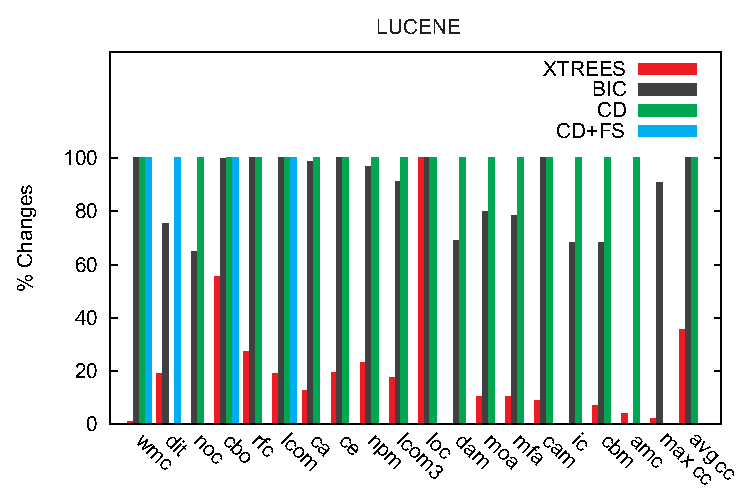
\includegraphics[width=0.9\linewidth]{_figs/Deltas-Lucene.eps}
\label{fig:delta_ivy}
\end{minipage}
\begin{minipage}{0.5\textwidth}
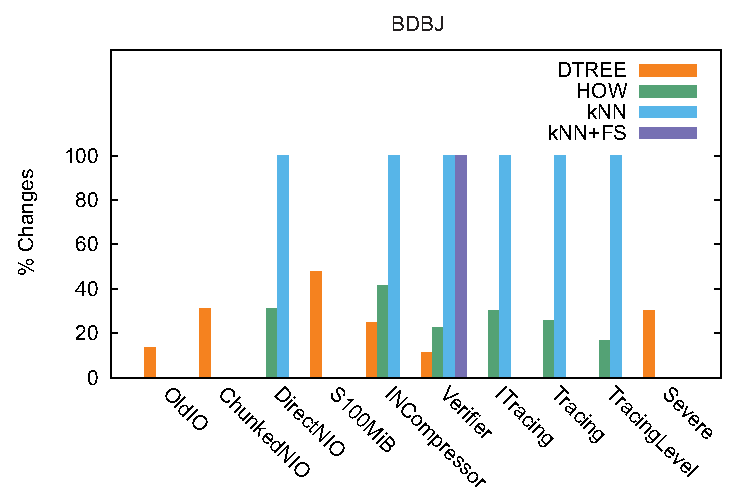
\includegraphics[width=0.9\linewidth]{_figs/Deltas-BDBJ.eps}
\label{fig:delta_apache}
\end{minipage}
\caption{Performance Comparison showing the number of times a certain feature requires to be changed. X-axis lists the various features that make up a data set. The y-axis contains the frequency of change in \%.}
\end{figure}

The clear advantage of our current work is that it can be readily and automatically applied to domains with historical data. However, the obvious drawback with this approach is that our assessment of the plans is only as good as the predictor. To mitigate for this {\em problem of poor predictors}, it is wise to demand certain standards for {\em satisfactory} thresholds. 

For the Jureczko OO data sets, we found:
\bi
\item
Most predictors in this domain were far from perfect;
\item 
But several of these predictors could
be salvaged using some sampling and optimization methods (see the notes on SMOTE and differential evolution, below).
\ei
As shown in \fig{j}, we   explore numerous examples of the Jureczko   object-oriented static code data sets: Ant, Camel, Ivy, Jedit,   Log4, Lucene, Poi, Synapse, Velocity, Xalan, Xerces\footnote{Available from the object-oriented defects section of the PROMISE respository~\cite{promiserepo}.}. 
Given access to $V$ released
versions, we test on version $V$ and train on the available data from $V-1$ earlier releases (as
shown in \fig{j}, this means that we are training on hundreds to thousands
of classes and testing on smaller test suites).
Note the three bottom rows marked with $\times$: these contain predominately
defective classes (two-thirds, or more) and in such data sets, it is hard to distinguish
good from bad (since there are so many bad examples). 

For the  Jureczko   data,
the plans generated by our planners advise on  how to change static code attributes in order to reduce defects in Java classes. Here, prediction performance of Random Forest can be measured using:
\bi
\item Probability of detection (a.k.a. ``pd'' or recall):  the percent of faulty classes in
the test data detected
by the {\em predictor}.
\item Probability of false alarm (a.k.a. ``pf''): the percent of non-fault
classes that are {\em predicted} to be defective.
\ei 

The ``untuned'' columns of \fig{j} shows Random Forest's {\em pd,pf}
values generated after learning from the training data and then being applied to the test data.
If we define ``good'' to mean $\mathit{pd}>60 \wedge \mathit{pf} < 40$\%,
then only two of our data sets ({\em ivy,ant}) are ``good'' enough. 

However, the ``tuned'' columns of \fig{j} show that we can salvage some of the data sets. Pelayo and Dick~\cite{pelayo07} report that defect prediction is improved by SMOTE~\cite{Chawla2002}; i.e. an over-sampling of minority-class examples. Also, Fu et al.~\cite{fu:fse16} report that parameter tuning with differential evolution~\cite{storn97} can quickly explore the tuning options of Random Forest to find better settings for the (e.g.) size of the forest, the termination criteria
for tree generation, etc. The rows marked with $\star$ in \fig{j} show data sets whose performance was improved remarkably by these techniques. For example, in {\em poi}, the recall increased by 4\% while the false alarm rate dropped by 21\%. However,  as might have been expected, we could not salvage the data sets in the  three bottom rows.

Turning now to the Seigmund data, the lessons learnt from the planners advise on how  to change the configurations settings within a Makefile (in order to make resulting compiled code  run faster). Here, performance can be measured in terms of  difference between the predicted runtime $p$ of test case items and their actual runtimes $a$ using  $s=\frac{abs(a - p)}{a}$.

This paper  explores six Seigmund configuration data sets:  Berkeley DB (Java and C versions), Apache, SQLite, LLVM, and
  x264\footnote{Available from the performance prediction section of PROMISE
  http://openscience.us/repo/performance-predict.}. 
  After splitting that data into equal sized train:test groups, a Random Forest
  Regressor trained on one half, then applied to the other, achieved nearly perfect scores of \[s=\{99.9, 99.8, 99.4, 99.1, 96.1\}\] 
  
That is, we can be very confident that the predictors from the Seigmund data can assess
our plans. (Aside: if the reader doubts that such high scores are achievable, we note that these scores are consistent with those achieved by predictors built by Seigmund et al.~\cite{sven12}.)

In summary, while we cannot trust predictors from some of our defect data sets,
we can plan ways to reduce defects in {\em jedit, ivy, ant, lucene} and {\em poi}.
One important detail to be stressed here is that, when we applied    SMOTE-ing and
parameter tunings, those techniques were applied to the training data and {\em not}
the test data; i.e. we took care that no clues from the test set were ever used in this tuning process.

\subsection{Assessment}
\fig{work} showed how we build and test our planners. The dependent variables of Jureczko and Seigmund data sets are discrete and continuous in nature, respectively. Hence, while choosing the predictor, we used Random Forest (1) as a classifier for Jureczko data and (2) as a regressor for Seigmund data. Additionally, for both the data sets, we designed a setup that repeated the trials 40 times (the value 40 was chosen to satisfy the minimum sample size requirements of the central limit theorem):
\bi
\item For Seigmund data, we randomized the order of the data, training on one half while identifying treatment plans on the remaining test data.
\item For the Jureczko data, we used the training and testing sets of \fig{j}. 
\ei
The 40 repeats defined above were repeated for each planner. A Scott-Knott procedure was used to test for statistical differences in the result. The Scott-Knott procedure was recommended by Mittas \& Angelis in their 2013 IEEE TSE paper~\cite{mittas13}.

This method
sorts a list of $l$ treatments with $ls$ measurements by their median
score. It then
splits $l$ into sub-lists $m,n$ in order to maximize the expected value of
 differences  in the observed performances
before and after divisions. E.g. for lists $l,m,n$ of size $ls,ms,ns$ where $l=m\cup n$:
 $E(\Delta)=\frac{ms}{ls}abs(m.\mu - l.\mu)^2 + \frac{ns}{ls}abs(n.\mu - l.\mu)^2$.
Scott-Knott  applies an  hypothesis test $H$ to check
if $m,n$ are significantly different. If so, Scott-Knott  recurses on the splits.

The hypothesis test $H$ used here is a conjunction of the A12 effect size test and a non-parametric bootstrap sampling. In other words, the Scott-Knott procedure being used here divides the data if \textit{both} bootstrap sampling and effect size test agree that a division is statistically significant (with a confidence of 99\%) and not a small effect ($A12 \ge 0.6$). For a justification of the use of non-parametric bootstrapping, see Efron \& Tibshirani~\cite[p220-223]{efron93}. For a justification of the use of effect size tests see Shepperd\&MacDonell~\cite{shepperd12a}; Kampenes~\cite{kampenes07}; and Kocaguenli et al.~\cite{Kocaguneli2013:ep}. These researchers warn that even if an hypothesis test declares two populations to be ``significantly'' different, then that result is misleading if the ``effect size'' is very small. Hence, to assess the performance differences we first must rule out small effects using A12, a test   recently endorsed by Arcuri and Briand at ICSE'11~\cite{arcuri11}.

\subsection{Results}
\begin{figure}[!t]
\centering
{\small
\begin{tabular}{lcccc}
  \hline
  \rowcolor{lightgray}
       & DTREE & HOW   & kNN   & kNN+FS \\\hline
Ant    & 20.24\% & 86.84\% & 80.00\% & 10.00\%  \\
Ivy    & 20.88\% & 81.25\% & 70.00\% & 20.00\%  \\
Jedit  & 19.55\% & 92.27\% & 90.00\% & 20.00\%  \\
Lucene & 18.92\% & 85.64\% & 95.00\% & 25.00\%  \\
Poi    & 12.90\% & 79.45\% & 85.00\% & 20.00\%   \\\hline
\end{tabular}}
\noindent
\caption{Average change in attribute values}\label{fig:types}
\end{figure}
The results for each data, for different planners, are shown in \fig{jur} and \fig{conf}. All
\subsection{Discussion}
\section{Threats to Validity}
\begin{figure}[!t]
%\noindent\begin{minipage}{0.5\textwidth} 
{\small 
\begin{tabular}{llrrc}
\arrayrulecolor{lightgray}
\rowcolor{lightgray}\textbf{Rank} & \textbf{Treatment} & \textbf{Median} & \textbf{IQR} & \\\hline
  1 &        XTREE &   59   &  9 & \quart{75}{4}{78}{99} \\
\hline   2 &      BIC &    5  & 1  & \quart{44}{0}{44}{99} \\
2 &          CD+FS & -7  & 100  & \quart{0}{53}{43}{99} \\   
2 &      CD &    -9  &  77 & \quart{21}{41}{42}{99} \\
\hline \end{tabular}}
\caption{Methods 1,2,3,4 applied to some ground-truth data (in this case, the POM3 model).
Values collected from  40 repeated runs of each method with different random seeds.
Results show the efficacy of XTREE in reducing the total overall cost in the original test data, when other planners fail to do so.}\label{fig:coc}
\end{figure}
\section{Conclusion}
\section*{Acknowledgements}
\bibliographystyle{plain}

\bibliography{References}
\end{document}
